\section{Conclusion}

\subsection{Privacy, Reliability, and Scalability}

This paper explained how the HOPR protocol, particularly its proof-of-relay mechanism, provides a first solution to building a scalable and robust incentivized network which provides full anonymity with minimal trade-offs in latency and bandwidth. Although HOPR is indebted to previous developments in the space, particularly the Sphinx packet format and the Ethereum blockchain, we believe its unique combination of probabilistic payments and verifiable but unlinkable cryptographic tickets is the first viable approach to creating a global privacy network which does not rely on any centralized entity to provide data transmission or incentive management.

The HOPR protocol is still under active development, with much research and implementation work still to be completed, but a working proof of concept is already live and available to use. 

\subsection{Future work}

\subsubsection{Path position leak}

In HOPR, payments are performed at each hop along a packet’s route. These
incentives weaken the unlinkability guarantees inherited from the Sphinx packet
format \cite{sphinxpaper} as they reveal the identity of the packet sender, who
must transfer these incentives using their signature. To solve this
problem, HOPR forwards incentives along with the packet.

\begin{figure}[H]
    \centering
    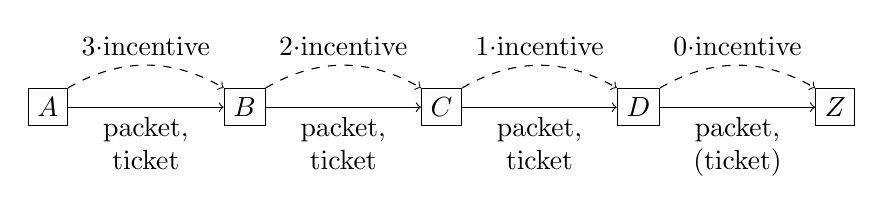
\begin{tikzpicture}[auto]
        \draw (0,0) node (a) [rectangle,draw] {$A$};
        \draw (2.5,0) node (b) [rectangle,draw] {$B$};
        \draw (5,0) node (c) [rectangle,draw] {$C$};
        \draw (7.5,0) node (d) [rectangle,draw] {$D$};
        \draw (10,0) node (z) [rectangle,draw] {$Z$};

        \draw [->,draw] (a.east) to node [align=center,below] {packet,\\ticket} (b.west);
        \draw [->,draw] (b.east) to node [align=center,below] {packet,\\ticket} (c.west);
        \draw [->,draw] (c.east) to node [align=center,below] {packet,\\ticket} (d.west);
        \draw [->,draw] (d.east) to node [align=center,below] {packet,\\(ticket)}  (z.west);

        \path [->,draw,bend left,dashed] (a.north east) to node [above] {3$\cdot$incentive} (b.north west);
        \path [->,draw,bend left,dashed] (b.north east) to node [above] {2$\cdot$incentive} (c.north west);
        \path [->,draw,bend left,dashed] (c.north east) to node [above] {1$\cdot$incentive} (d.north west);
        \path [->,draw,bend left,dashed] (d.north east) to node [above] {0$\cdot$incentive} (z.north west);

    \end{tikzpicture}
    \caption{Incentive workflow}
    \label{fig:incentive worklow}
\end{figure}

However, this leaks the relayer’s position within the selected path, since the value of the ticket is set according to the current relay fee and the
number of intermediate hops, more precisely $$amount:=\frac{(hops -1)* relayFee}{winProb}$$
This leak is considered low severity, but further research will be
conducted on the subject.

\subsubsection{Reputation (aggregated trust matrix)}

In HOPR, we assume the majority of nodes are honest and act properly.
Nevertheless, there might be nodes who actively try to attack the network by:

\begin{itemize}

    \item Dropping packets or acknowledgements

    \item Sending false packets, tickets, or acknowledgements

\end{itemize}

Since nodes need to monitor the network to select paths, they need to filter
nodes that behave inappropriately. To help nodes achieve this, HOPR is considering implementing a
transitive reputation system which assigns a score to each node that acts as a
relayer. A node’s behaviour will affect its reputation, which will in turn affect its probability of
being chosen as a relayer.

\subsubsection*{Transitive trust evaluation }

Reputation within a network can be defined as ``a peer’s belief in another peer’s
capabilities, honesty, and reliability based on other peers recommendations” \cite{Wang_2003}.
Trust is represented by a triplet (trust, distrust, uncertainty) where:

\begin{itemize}

    \item Trust: $td^t(d,e,x,k)=\frac{n}{m}$ where $m$ is the number of all
        experiences and $n$ are the positive ones

    \item Distrust: $tdd^t(d,e,x,k)=\frac{l}{m}$ where $l$ stands for the number
        of the trustor’s negative experience.

    \item Uncertainty = 1 - trust - distrust.
 
 \subsubsection*{Commitment derivation}
  In the future $comm_0$ will be derived from the private key of the node as $$ comm_0 = \mathsf{h}(privKey,chainId,
contractAddr, channelId, channelEpoch)$$
And there will be further research to determine whether such a design leaks information about the
private key or not. 

\end{itemize}
